\documentclass[12pt,a4paper]{article}
\usepackage[utf8]{vietnam}
\usepackage{amsmath,amssymb}
\usepackage{tabularx}
\usepackage{graphicx}
\usepackage{tikz}
\usetikzlibrary{calc,arrows.meta}
\usepackage{xcolor}
\usepackage{enumitem}
\usepackage{fancyhdr}
\usepackage[top=1.0cm, bottom=1.0cm, left=1.3cm, right=1.3cm]{geometry}
\usepackage[loigiai]{ex_test}
\SAOPTN{widthSA=2.6,heightSA=0.62}

\setlength{\headheight}{15pt}
\setlength{\parskip}{1pt}

\pagestyle{fancy}
\fancyhf{}
\rhead{\textit{Lời giải chi tiết -- Đề số 12}}
\lhead{\textit{Bộ đề ôn tập Giữa học kì I -- Toán 7}}
\cfoot{\thepage}

\begin{document}

\begin{center}
\textbf{\Large HƯỚNG DẪN CHẤM VÀ LỜI GIẢI CHI TIẾT}\\
\vspace{1mm}
\textbf{\large MÔN: TOÁN 7 -- ĐỀ SỐ 12}
\end{center}
\vspace{2mm}

\noindent\textbf{\large PHẦN I. CÂU TRẮC NGHIỆM NHIỀU PHƯƠNG ÁN LỰA CHỌN}

\vspace{1mm}
\begin{ex}
Kết quả của phép tính $-\dfrac{7}{8} - \dfrac{5}{4}$ là:
\choice
{$\dfrac{3}{8}$}
{$\dfrac{17}{8}$}
{$-\dfrac{3}{8}$}
{\True $-\dfrac{17}{8}$}
\loigiai{
Quy đồng mẫu số hai phân số: $-\dfrac{7}{8} - \dfrac{5}{4} = -\dfrac{7}{8} - \dfrac{10}{8} = \dfrac{-7 - 10}{8} = -\dfrac{17}{8}$.
}
\end{ex}

\begin{ex}
Các mặt bên của hình lăng trụ đứng tam giác là:
\choice
{Các hình tam giác}
{\True Các hình chữ nhật}
{Các hình thang cân}
{Các hình vuông}
\loigiai{
Theo định nghĩa hình lăng trụ đứng tam giác, các mặt bên luôn là các hình chữ nhật.
}
\end{ex}

\begin{ex}
Một hình lập phương có cạnh $a = 5\text{ cm}$. Diện tích xung quanh của hình lập phương đó là:
\choice
{$25\text{ cm}^2$}
{$50\text{ cm}^2$}
{\True $100\text{ cm}^2$}
{$150\text{ cm}^2$}
\loigiai{
Diện tích xung quanh hình lập phương cạnh $a$: $S_{xq} = 4a^2 = 4 \cdot 5^2 = 4 \cdot 25 = 100\text{ cm}^2$.
}
\end{ex}

\begin{ex}
Trong các số sau, số nào là số vô tỉ?
\choice
{$\sqrt{9}$}
{$\dfrac{3}{2}$}
{$2{,}5$}
{\True $\sqrt{5}$}
\loigiai{
Ta có $\sqrt{9} = 3 \in \mathbb{Q}$, $\dfrac{3}{2} \in \mathbb{Q}$, $2{,}5 = \dfrac{5}{2} \in \mathbb{Q}$. Còn $\sqrt{5} = 2{,}2360679...$ là số thập phân vô hạn không tuần hoàn nên $\sqrt{5}$ là số vô tỉ.
}
\end{ex}

\begin{ex}
\immini{
Cho hình lăng trụ đứng tam giác $ABC.A'B'C'$ (như hình vẽ bên). Các mặt bên của hình trên là những hình gì?
\choice
{Tam giác}
{Hình thoi}
{\True Hình chữ nhật}
{Hình bình hành}
}{
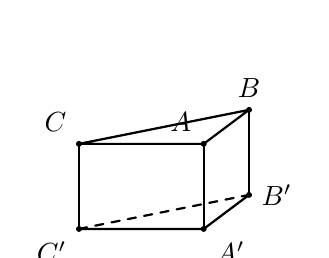
\begin{tikzpicture}[scale=0.72, line cap=round, line join=round]
    \coordinate (C) at (0, 1.5);
    \coordinate (A) at (2.2, 1.5);
    \coordinate (B) at (3.0, 2.1);
    \coordinate (C_prime) at (0, 0);
    \coordinate (A_prime) at (2.2, 0);
    \coordinate (B_prime) at (3.0, 0.6);

    \draw[thick] (C) -- (A) -- (B) -- (C);
    \draw[thick] (C) -- (C_prime);
    \draw[thick] (A) -- (A_prime);
    \draw[thick] (B) -- (B_prime);
    \draw[thick] (C_prime) -- (A_prime) -- (B_prime);
    \draw[thick, dashed] (C_prime) -- (B_prime);

    \filldraw[black] (C) circle (1.2pt) node[above left=1pt] {$C$};
    \filldraw[black] (A) circle (1.2pt) node[above left=1pt] {$A$};
    \filldraw[black] (B) circle (1.2pt) node[above=1pt] {$B$};
    \filldraw[black] (C_prime) circle (1.2pt) node[below left=1pt] {$C'$};
    \filldraw[black] (A_prime) circle (1.2pt) node[below right=1pt] {$A'$};
    \filldraw[black] (B_prime) circle (1.2pt) node[right=1pt] {$B'$};
\end{tikzpicture}
}
\loigiai{
Các mặt bên của hình lăng trụ đứng tam giác ($ABB'A', BCC'B', ACC'A'$) là các hình chữ nhật.
}
\end{ex}

\begin{ex}
Số nào trong các số dưới đây không là số hữu tỉ?
\choice
{\True $\dfrac{3}{0}$}
{$0{,}625$}
{$\dfrac{0}{3}$}
{$2\dfrac{3}{5}$}
\loigiai{
Số hữu tỉ có dạng $\dfrac{a}{b}$ với $a, b \in \mathbb{Z}$ và $b \neq 0$. Phân số $\dfrac{3}{0}$ có mẫu số bằng $0$ nên không phải là số hữu tỉ.
}
\end{ex}

\begin{ex}
Tích $(-3{,}1) \cdot (-3{,}1) \cdot (-3{,}1) \cdot (-3{,}1) \cdot (-3{,}1)$ viết gọn là:
\choice
{$(-3{,}1) \cdot 5$}
{\True $(-3{,}1)^5$}
{$(3{,}1)^5$}
{$3{,}1 \cdot 5$}
\loigiai{
Tích của 5 thừa số $(-3{,}1)$ bằng lũy thừa bậc 5 của $(-3{,}1)$, tức là $(-3{,}1)^5$.
}
\end{ex}

\begin{ex}
Kết quả của phép tính $\dfrac{4}{7} - \dfrac{5}{9}$ bằng:
\choice
{\True $\dfrac{1}{63}$}
{$\dfrac{2}{63}$}
{$\dfrac{4}{63}$}
{$\dfrac{5}{63}$}
\loigiai{
Quy đồng mẫu số chung 63: $\dfrac{4}{7} - \dfrac{5}{9} = \dfrac{36}{63} - \dfrac{35}{63} = \dfrac{1}{63}$.
}
\end{ex}

\begin{ex}
\immini{
Cho điểm $O$ thuộc đường thẳng $AB$. Số đo $\widehat{BOC}$ trong hình vẽ bên là:
\choice
{\True $60^\circ$}
{$120^\circ$}
{$180^\circ$}
{$90^\circ$}
}{
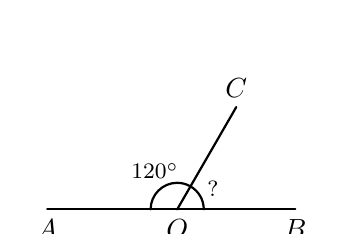
\begin{tikzpicture}[scale=0.75, line cap=round, line join=round]
    \coordinate (O) at (0,0);
    \coordinate (A) at (-2.2,0);
    \coordinate (B) at (2.0,0);
    \coordinate (C) at (60:2.0);
    \draw[thick] (A) -- (B);
    \draw[thick] (O) -- (C);
    \node[below] at (A) {$A$};
    \node[below] at (O) {$O$};
    \node[below] at (B) {$B$};
    \node[above] at (C) {$C$};
    \draw[thick] (O) ++(180:0.45) arc (180:60:0.45);
    \node[font=\footnotesize] at (120:0.75) {$120^\circ$};
    \draw[thick] (O) ++(60:0.45) arc (60:0:0.45);
    \node[font=\footnotesize] at (30:0.7) {$?$};
\end{tikzpicture}
}
\loigiai{
Do ba điểm $A, O, B$ thẳng hàng nên $\widehat{AOC}$ và $\widehat{BOC}$ là hai góc kề bù: $\widehat{BOC} = 180^\circ - \widehat{AOC} = 180^\circ - 120^\circ = 60^\circ$.
}
\end{ex}

\begin{ex}
Số nào dưới đây là số thập phân vô hạn tuần hoàn?
\choice
{$0{,}123123$}
{$\dfrac{1}{2}$}
{\True $0{,}(3)$}
{$0{,}3$}
\loigiai{
Số $0{,}(3) = 0{,}333...$ có phần thập phân lặp lại chu kỳ 3 vô hạn nên là số thập phân vô hạn tuần hoàn.
}
\end{ex}

\begin{ex}
Cho $\widehat{xOy} = 70^\circ$. Góc đối đỉnh với $\widehat{xOy}$ có số đo bằng:
\choice
{$110^\circ$}
{\True $70^\circ$}
{$180^\circ$}
{$35^\circ$}
\loigiai{
Hai góc đối đỉnh thì bằng nhau, do đó góc đối đỉnh với $\widehat{xOy}$ cũng bằng $70^\circ$.
}
\end{ex}

\begin{ex}
Một hình hộp chữ nhật có chiều dài $6\text{ cm}$, chiều rộng $4\text{ cm}$ và chiều cao $5\text{ cm}$. Thể tích của hình hộp chữ nhật đó là:
\choice
{\True $120\text{ cm}^3$}
{$74\text{ cm}^3$}
{$60\text{ cm}^3$}
{$120\text{ cm}^2$}
\loigiai{
Áp dụng công thức thể tích hình hộp chữ nhật $V = a \cdot b \cdot h = 6 \cdot 4 \cdot 5 = 120\text{ cm}^3$.
}
\end{ex}


\setcounter{ex}{0}
\noindent\textbf{\large PHẦN II. CÂU TRẮC NGHIỆM ĐÚNG SAI}

\vspace{1mm}
\begin{ex}
Cho biểu thức $X = \left(-\dfrac{3}{2}\right)^2 - \dfrac{5}{4} \cdot \left(-\dfrac{2}{5}\right) + \left(-\dfrac{1}{4}\right)$. Xét tính đúng sai của các mệnh đề sau:
\choiceTF
{\True Giá trị của lũy thừa $\left(-\dfrac{3}{2}\right)^2$ bằng $\dfrac{9}{4}$}
{\True Giá trị của phép nhân $\dfrac{5}{4} \cdot \left(-\dfrac{2}{5}\right)$ bằng $-\dfrac{1}{2}$}
{Giá trị của biểu thức $X$ bằng $3$}
{Giá trị $X$ thu được là một số nguyên âm}
\loigiai{
\begin{itemize}[leftmargin=0.6cm, itemsep=1pt]
\item \textbf{a)} \textbf{Đúng}. Ta có $\left(-\dfrac{3}{2}\right)^2 = \dfrac{(-3)^2}{2^2} = \dfrac{9}{4}$.
\item \textbf{b)} \textbf{Đúng}. Ta có $\dfrac{5}{4} \cdot \left(-\dfrac{2}{5}\right) = -\dfrac{5 \cdot 2}{4 \cdot 5} = -\dfrac{2}{4} = -\dfrac{1}{2}$.
\item \textbf{c)} \textbf{Sai}. Ta có $X = \dfrac{9}{4} - \left(-\dfrac{1}{2}\right) + \left(-\dfrac{1}{4}\right) = \dfrac{9}{4} + \dfrac{2}{4} - \dfrac{1}{4} = \dfrac{10}{4} = \dfrac{5}{2} = 2{,}5 \neq 3$.
\item \textbf{d)} \textbf{Sai}. Giá trị $X = \dfrac{5}{2} > 0$ là một số hữu tỉ dương, không phải số nguyên âm.
\end{itemize}
}
\end{ex}

\begin{ex}
\immini{
Quan sát hình lăng trụ đứng tam giác $ABC.A'B'C'$ dưới đây. Xét tính đúng sai của các mệnh đề sau:
\choiceTF
{\True Hai mặt đáy của hình lăng trụ đứng là tam giác $ABC$ và tam giác $A'B'C'$}
{Các mặt bên $ABB'A', BCC'B', ACC'A'$ là các hình tam giác}
{\True Các cạnh bên $AA', BB', CC'$ song song và bằng nhau}
{\True Nếu đáy $ABC$ là tam giác vuông tại $A$ có $AB = 3\text{ cm}, AC = 4\text{ cm}$ và chiều cao $AA' = 5\text{ cm}$ thì thể tích của hình lăng trụ bằng $30\text{ cm}^3$}
}{
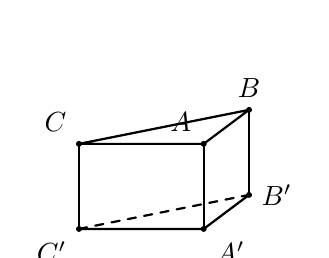
\begin{tikzpicture}[scale=0.72, line cap=round, line join=round]
    \coordinate (C) at (0, 1.5);
    \coordinate (A) at (2.2, 1.5);
    \coordinate (B) at (3.0, 2.1);
    \coordinate (C_prime) at (0, 0);
    \coordinate (A_prime) at (2.2, 0);
    \coordinate (B_prime) at (3.0, 0.6);

    \draw[thick] (C) -- (A) -- (B) -- (C);
    \draw[thick] (C) -- (C_prime);
    \draw[thick] (A) -- (A_prime);
    \draw[thick] (B) -- (B_prime);
    \draw[thick] (C_prime) -- (A_prime) -- (B_prime);
    \draw[thick, dashed] (C_prime) -- (B_prime);

    \filldraw[black] (C) circle (1.2pt) node[above left=1pt] {$C$};
    \filldraw[black] (A) circle (1.2pt) node[above left=1pt] {$A$};
    \filldraw[black] (B) circle (1.2pt) node[above=1pt] {$B$};
    \filldraw[black] (C_prime) circle (1.2pt) node[below left=1pt] {$C'$};
    \filldraw[black] (A_prime) circle (1.2pt) node[below right=1pt] {$A'$};
    \filldraw[black] (B_prime) circle (1.2pt) node[right=1pt] {$B'$};
\end{tikzpicture}
}
\loigiai{
\begin{itemize}[leftmargin=0.6cm, itemsep=1pt]
\item \textbf{a)} \textbf{Đúng}. Hai mặt đáy là hai tam giác song song và bằng nhau: tam giác $ABC$ và tam giác $A'B'C'$.
\item \textbf{b)} \textbf{Sai}. Các mặt bên của hình lăng trụ đứng tam giác là các hình chữ nhật.
\item \textbf{c)} \textbf{Đúng}. Theo tính chất hình lăng trụ đứng, các cạnh bên luôn song song và bằng nhau.
\item \textbf{d)} \textbf{Đúng}. Diện tích đáy là $S_{\text{đáy}} = \dfrac{1}{2} \cdot AB \cdot AC = \dfrac{1}{2} \cdot 3 \cdot 4 = 6\text{ cm}^2$. Thể tích lăng trụ: $V = S_{\text{đáy}} \cdot h = 6 \cdot 5 = 30\text{ cm}^3$.
\end{itemize}
}
\end{ex}


\setcounter{ex}{0}
\noindent\textbf{\large PHẦN III. CÂU HỎI TRẢ LỜI NGẮN}

\vspace{1mm}
\begin{ex}
Tìm số tự nhiên $x$, biết: $3^{x+2} - 3^x = 216$. \shortans{3}
\loigiai{
Ta có: $3^{x+2} - 3^x = 216 \iff 3^x \cdot 3^2 - 3^x = 216 \iff 3^x \cdot (9 - 1) = 216 \iff 3^x \cdot 8 = 216 \iff 3^x = 27 \iff 3^x = 3^3 \iff x = 3$.

\textbf{Đáp số:} $3$
}
\end{ex}

\begin{ex}
Cho hai đường thẳng song song $a$ và $b$. Đường thẳng $c$ cắt $a$ và $b$ lần lượt tại hai điểm $A$ và $B$. Biết $\widehat{A}_1$ và $\widehat{B}_1$ là hai góc trong cùng phía và $\widehat{A}_1 = 2\widehat{B}_1$. Tính số đo góc $\widehat{A}_1$. \shortans{$120^\circ$}
\loigiai{
Vì $a \parallel b$ nên hai góc trong cùng phía $\widehat{A}_1$ và $\widehat{B}_1$ bù nhau: $\widehat{A}_1 + \widehat{B}_1 = 180^\circ$. Thay $\widehat{A}_1 = 2\widehat{B}_1$, ta được $2\widehat{B}_1 + \widehat{B}_1 = 180^\circ \iff 3\widehat{B}_1 = 180^\circ \iff \widehat{B}_1 = 60^\circ$. Suy ra $\widehat{A}_1 = 2 \cdot 60^\circ = 120^\circ$.

\textbf{Đáp số:} $120^\circ$
}
\end{ex}


\setcounter{ex}{0}
\noindent\textbf{\large PHẦN IV. TỰ LUẬN}

\vspace{1mm}
\begin{ex}
Tính hợp lý (nếu có):
\begin{enumerate}[label=\textbf{\alph*)}, leftmargin=0.8cm, itemsep=1pt]
\item $\dfrac{1}{6} - \dfrac{2}{5}$
\item $\left(-\dfrac{1}{3}\right)^2 : \dfrac{5}{9} + (-1)^{2024}$
\item $\left(\dfrac{5}{171} + \dfrac{8}{3}\right) - \left(-\dfrac{5}{3} - \dfrac{5}{171}\right) - 1\dfrac{2}{5}$
\end{enumerate}
\loigiai{
\textbf{a)} $\dfrac{1}{6} - \dfrac{2}{5} = \dfrac{5}{30} - \dfrac{12}{30} = -\dfrac{7}{30}$.

\textbf{b)} $\left(-\dfrac{1}{3}\right)^2 : \dfrac{5}{9} + (-1)^{2024} = \dfrac{1}{9} : \dfrac{5}{9} + 1 = \dfrac{1}{9} \cdot \dfrac{9}{5} + 1 = \dfrac{1}{5} + 1 = \dfrac{6}{5}$.

\textbf{c)} Ta có: $\left(\dfrac{5}{171} + \dfrac{8}{3}\right) - \left(-\dfrac{5}{3} - \dfrac{5}{171}\right) - \dfrac{7}{5} = \dfrac{5}{171} + \dfrac{8}{3} + \dfrac{5}{3} + \dfrac{5}{171} - \dfrac{7}{5} = \left(\dfrac{5}{171} + \dfrac{5}{171}\right) + \left(\dfrac{8}{3} + \dfrac{5}{3}\right) - \dfrac{7}{5}$... Nhận thấy theo đề gốc số hạng thứ nhất là $-\dfrac{5}{171}$: $\left(-\dfrac{5}{171} + \dfrac{8}{3}\right) - \left(-\dfrac{5}{3} - \dfrac{5}{171}\right) - \dfrac{7}{5} = \left(-\dfrac{5}{171} + \dfrac{5}{171}\right) + \left(\dfrac{8}{3} + \dfrac{5}{3}\right) - \dfrac{7}{5} = 0 + \dfrac{13}{3} - \dfrac{7}{5} = \dfrac{65 - 21}{15} = \dfrac{44}{15}$. Hoặc nếu là $\dfrac{8}{3} - \dfrac{5}{3} = 1$: $0 + 1 - \dfrac{7}{5} = -\dfrac{2}{5}$.
}
\end{ex}
\vspace{2mm}

\begin{ex}
Tìm $x$, biết:
\begin{enumerate}[label=\textbf{\alph*)}, leftmargin=0.8cm, itemsep=1pt]
\item $\dfrac{1}{3} + \dfrac{2}{3} : x = -7$
\item $(x - 2{,}5)^2 = 16$
\end{enumerate}
\loigiai{
\textbf{a)} $\dfrac{2}{3} : x = -7 - \dfrac{1}{3} \iff \dfrac{2}{3} : x = -\dfrac{22}{3} \iff x = \dfrac{2}{3} : \left(-\dfrac{22}{3}\right) \iff x = \dfrac{2}{3} \cdot \left(-\dfrac{3}{22}\right) \iff x = -\dfrac{1}{11}$. Vậy $x = -\dfrac{1}{11}$.

\textbf{b)} Vì $4^2 = 16$ và $(-4)^2 = 16$, ta xét hai trường hợp:\par $\bullet$ TH1: $x - 2{,}5 = 4 \iff x = 4 + 2{,}5 \iff x = 6{,}5$.\par $\bullet$ TH2: $x - 2{,}5 = -4 \iff x = -4 + 2{,}5 \iff x = -1{,}5$.\par Vậy $x = 6{,}5$ hoặc $x = -1{,}5$.
}
\end{ex}
\vspace{2mm}

\begin{ex}
\immini{
Cho hình vẽ bên, trong đó $Ax \parallel By$ và $\widehat{xAB} = 40^\circ, \widehat{ABC} = 105^\circ, \widehat{BCz} = 65^\circ$.
\begin{enumerate}[label=\textbf{\alph*)}, leftmargin=0.8cm, itemsep=1pt]
\item Tính số đo $\widehat{ABy}$.
\item Chứng minh rằng $By$ song song với $Cz$.
\item Kẻ $BD$ là tia phân giác của $\widehat{CBy}$ ($D \in Cz$). Tính số đo $\widehat{BDC}$.
\end{enumerate}
}{
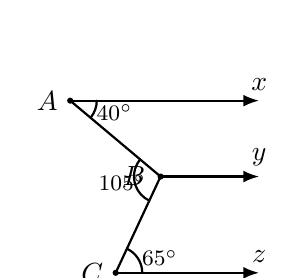
\begin{tikzpicture}[scale=0.75, line cap=round, line join=round]
    \coordinate (A) at (0, 2.4);
    \coordinate (x) at (3.2, 2.4);
    \coordinate (B) at (1.53, 1.115);
    \coordinate (y) at (3.2, 1.115);
    \coordinate (C) at (0.77, -0.515);
    \coordinate (z) at (3.2, -0.515);

    \draw[thick, -{Latex[length=2mm]}] (A) -- (x) node[above] {$x$};
    \draw[thick, -{Latex[length=2mm]}] (B) -- (y) node[above] {$y$};
    \draw[thick, -{Latex[length=2mm]}] (C) -- (z) node[above] {$z$};
    \draw[thick] (A) -- (B) -- (C);

    \filldraw[black] (A) circle (1.2pt) node[left=1pt] {$A$};
    \filldraw[black] (B) circle (1.2pt) node[left=2pt] {$B$};
    \filldraw[black] (C) circle (1.2pt) node[left=1pt] {$C$};

    % Angles
    \draw[thick] (A) ++(0:0.45) arc (0:-40:0.45);
    \node[font=\footnotesize] at ($(A)+(0.75,-0.2)$) {$40^\circ$};

    \draw[thick] (B) ++(140:0.45) arc (140:245:0.45);
    \node[font=\footnotesize] at ($(B)+(-0.65,-0.1)$) {$105^\circ$};

    \draw[thick] (C) ++(0:0.45) arc (0:65:0.45);
    \node[font=\footnotesize] at ($(C)+(0.75,0.25)$) {$65^\circ$};
\end{tikzpicture}
}
\loigiai{
\textbf{a)} Vì $Ax \parallel By$ nên $\widehat{xAB}$ và $\widehat{ABy}$ là hai góc trong cùng phía:\par $\widehat{xAB} + \widehat{ABy} = 180^\circ \implies 40^\circ + \widehat{ABy} = 180^\circ \implies \widehat{ABy} = 180^\circ - 40^\circ = 140^\circ$.

\textbf{b)} Ta có tia $By$ nằm giữa hai tia $BA$ và $BC$ nên $\widehat{CBy} = 360^\circ - \widehat{ABy} - \widehat{ABC} = 360^\circ - 140^\circ - 105^\circ = 115^\circ$.\par Xét hai đường thẳng $By$ và $Cz$, hai góc $\widehat{CBy}$ và $\widehat{BCz}$ ở vị trí trong cùng phía có tổng: $\widehat{CBy} + \widehat{BCz} = 115^\circ + 65^\circ = 180^\circ$.\par Do đó $By \parallel Cz$.

\textbf{c)} Vì $BD$ là tia phân giác của $\widehat{CBy}$ nên $\widehat{DBy} = \dfrac{\widehat{CBy}}{2} = \dfrac{115^\circ}{2} = 57{,}5^\circ$.\par Vì $By \parallel Cz$ nên $\widehat{BDC}$ và $\widehat{DBy}$ ở vị trí so le trong, suy ra $\widehat{BDC} = \widehat{DBy} = 57{,}5^\circ$.
}
\end{ex}
\vspace{2mm}

\begin{ex}
Vào tháng 4, giá niêm yết của một chiếc laptop tại một cửa hàng máy tính là $16\,000\,000$ đồng. Đến tháng 8, cửa hàng giảm giá $10\%$ cho mỗi chiếc laptop. Sang tháng 10, cửa hàng lại giảm giá thêm một lần nữa, lúc này giá một chiếc laptop chỉ còn $13\,680\,000$ đồng. Hỏi tháng 10 cửa hàng đã giảm giá bao nhiêu phần trăm cho một chiếc laptop so với tháng 8?
\loigiai{
Giá của chiếc laptop trong tháng 8 sau khi giảm $10\%$ là:\par \centerline{$16\,000\,000 \cdot (100\% - 10\%) = 16\,000\,000 \cdot 0{,}9 = 14\,400\,000\text{ (đồng).}$}\par Số tiền cửa hàng đã giảm giá thêm trong tháng 10 là:\par \centerline{$14\,400\,000 - 13\,680\,000 = 720\,000\text{ (đồng).}$}\par Tỉ lệ phần trăm cửa hàng đã giảm giá trong tháng 10 so với tháng 8 là:\par \centerline{$\dfrac{720\,000}{14\,400\,000} \cdot 100\% = 5\%.$}\par Vậy tháng 10 cửa hàng đã giảm giá $5\%$ cho một chiếc laptop so với tháng 8.
}
\end{ex}
\vspace{2mm}


\begin{center}
\rule{4cm}{0.4pt}\\
\textit{--- HẾT ---}
\end{center}
\end{document}
